\begin{center}
	\hrule
	\vspace{.4cm}
	{\textbf { \large ELEC 300 --- Electric Circuits II}}
\end{center}
{\textbf{Name:}\ David Li \hspace{\fill} \textbf{Student Number:}} \ V00818631  \\
{\textbf{Due Date:} Monday, 29 January 2018, 11:30 AM \hspace{\fill} \textbf{Assignment:} Number 3 \\
	\hrule
	
%	\listoffigures
\paragraph{Problem 1}
\begin{figure}[h]
	\centering
	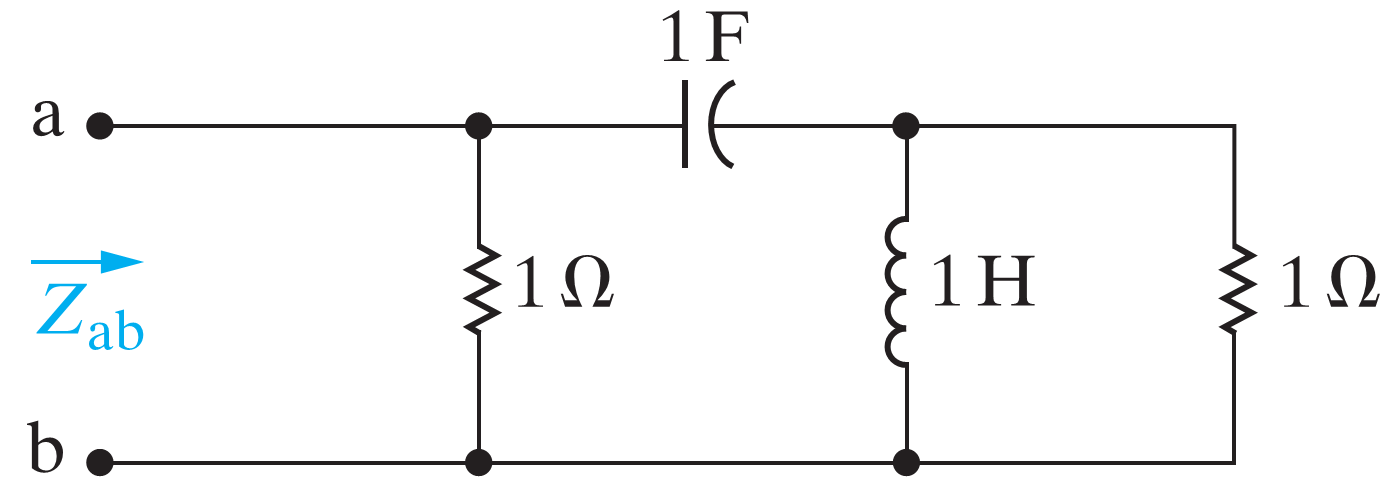
\includegraphics[width=1\linewidth]{images/Nil10th13-7}
	\caption{Problem 13-7 Nillison 10th edition}
	\label{fig:nil10th13-7}
\end{figure}
Find:
\begin{enumerate}[label=\alph*)]
	\item the input impedance as a fraction of polynomials in s
	Converting all values to the laplace domain and using basic circuit laws.
	\begin{align*}
	& Z_{ab}=\left( \left( s || 1\right) + \frac{1}{s} \right) || 1 \quad 
	s||1 = \frac{s}{s+1}, \quad 
	s||1 + \frac{1}{s}=\frac{s^2+s+1}{s(s+1)} \\
	& Z_{ab} = \cfrac{\frac{s^2+s+1}{s(s+1)}}{\frac{s^2+s+1}{s(s+1)}+1}= \frac{s^2+s+1}{2s^2+2s+1}=\frac{0.5(s^2+s+1)}{s^2+s+0.5} \Omega
	\end{align*}
	\item the poles and zeros of the impedance seen into terminals a-b.
	Using the quadratic equation
	\[
	Z_{ab} = \frac{0.5(s+0.5+j0.5\sqrt(3))(s+0.5-j0.5\sqrt(3))}{(s+0.5-j0.5)(s+0.5-j0.5)}
	\] 
\end{enumerate}

\paragraph{Problem 2}
Note that this is the wrong picture, however, just imagine that the current and switch don't exist, then the picture is good. %\smiley.
\begin{enumerate}[label=\alph*)]
	\item Find the transfer functions $H(s) =V_o(s)/V_i(s)$. Present the solution in the form of numerator and denominator polynomials in s.
	\item Derive a condition (involving circuit elements $R_1, R_2, C_1, C_2$) that leads to H(s) being independent of frequency. 
\end{enumerate}
\begin{figure}[H]
	\centering
	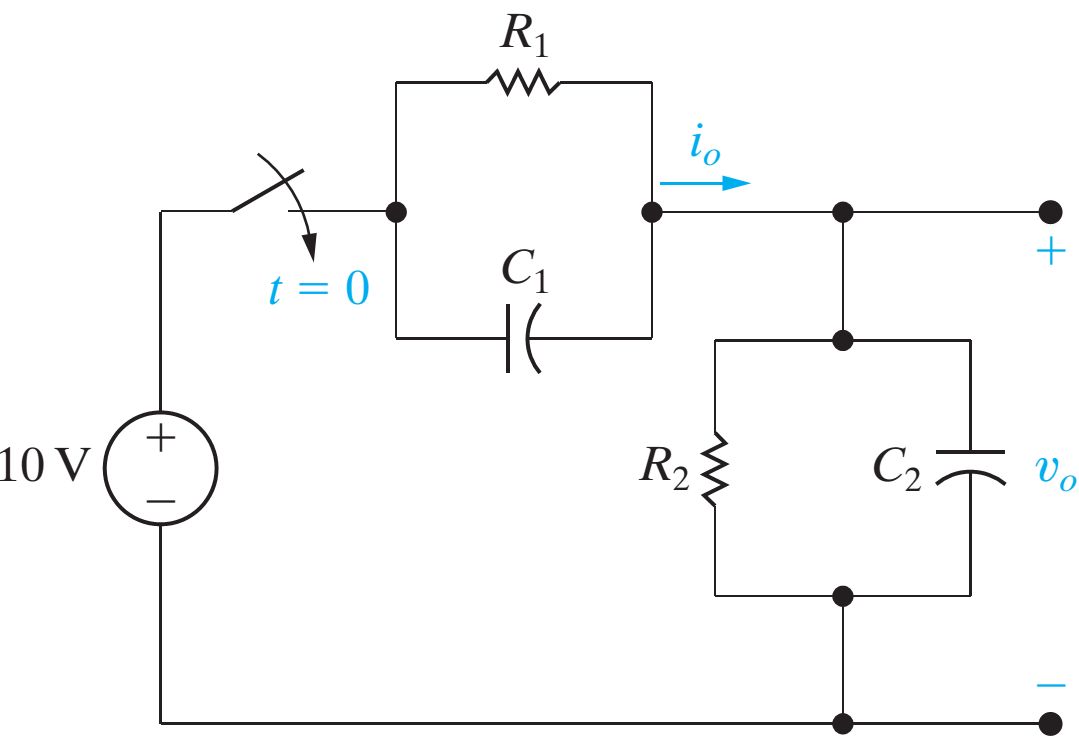
\includegraphics[width=1\linewidth]{images/Nil10th13-87}
	\caption{Problem 13-87 from Nillsion 10th edition}
	\label{fig:nil10th13-87}
\end{figure}
\paragraph{Problem 3}
A transfer function is given by
\[
T(s)= \cfrac{s+1}{s(s+10)}
\]
Sketch the straight-line magnitude and phase plots. 

\paragraph{Problem 4}
Sketch the straight-line magnitude and phase plots for
\[
H(s)=\cfrac{50(s+1)}{s(s^2+10s+100)}
\]
\paragraph{Problem 5}
The Bode magnitude plot belongs to a band reject filter that provides significant gain at low and high frequencies, but no gain to frequencies in the 10 to 50 rad/s range. Obtain the transfer function H(s). 


\begin{figure}[H]
	\centering
	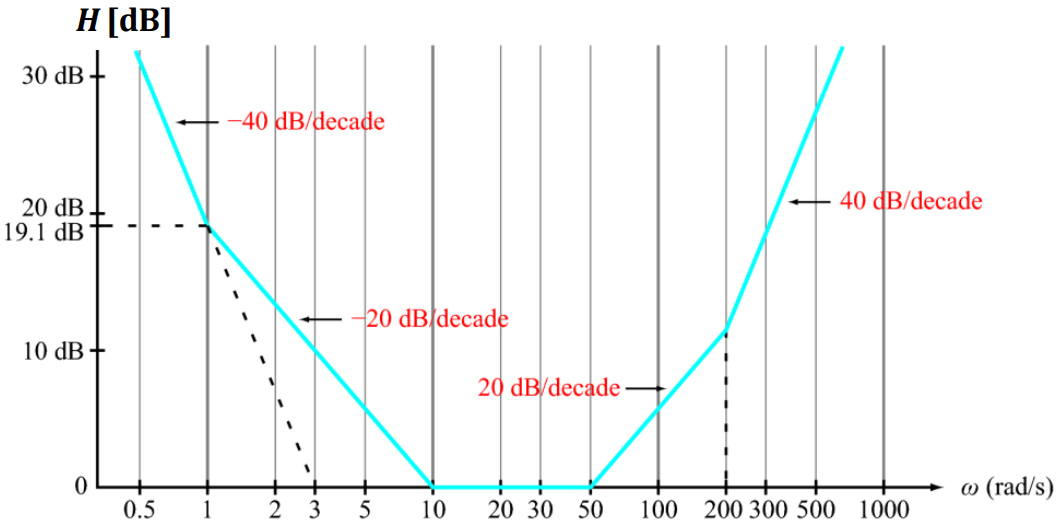
\includegraphics[width=1\linewidth]{images/ELEC300A3P5S2018.png}
	\caption{Problem 13-87 from Nillsion 10th edition}
	%\label{fig:nil10th13-87}
\end{figure}
\paragraph{Problem 6}
Problem 6
The general transfer function of a second-order bandpass filter is given by
\[
H(s)= \cfrac{}{s^2+2\zeta \omega_0 s + \omega_n^2}
\]
Find the transfer function H(s) of a passive (no Op-Amp) second-order bandpass filter with a center frequency of 20 kHz and a resonance peak of 20 dB above the straight-line approximation. 
%% Refer to matlab file for the rest of the work
Refer to matlab file for the rest of the work.